\section{Platformy SaaS z wbudowanym CI/CD}
\subsection{Z czego wynika popularność platform SaaS?}
Platformy takie jak GitHub, CircleCI czy też BitBucket zasłynęły z tego, że oferowały możliwość hostowania naszego repozytorium Git'owego w chmurze. Z biegiem czasu zaczęły one oferować dodatkowe usługi. Serwisy te to już nie tylko miejsce, które umożliwia hostowanie naszego repozytorium kodu - pozwalają one na takie rzeczy jak:
\begin{itemize}
    \item Odpalanie procesów automatyzujących (GitHub, GitLab, BitBucket) - dzięki możliwości tworzenia własnych procesów automatyzujących mamy możliwość zaimplementować własny proces ciągłej integracji, ciągłego dowożenia czy też ciągłego dostarczania,
    \item Odpalanie manualne predefiniowanych procesów (GitLab) - jest to dość prosta funkcjonalność, która daje sporo możliwości. GitLab dostarcza interfejs, w którym możemy uruchomić dowolny pipeline (z ang. \textit{potok}) manualnie - dodatkowo możemy podać argumenty w postaci pól tekstowych. Przykładem, gdzie ta funkcja GitLab'a byłaby użyteczna, jest aplikacja webowa, która zabiera dużo zasobów. Użycie procesu ciągłego dostarczania, by uruchamiać wersję staging'ową oznaczałoby, że aplikacja ta zbędnie używałaby zasoby na serwerze. Dzięki funkcji odpalania manualnego pipeline'ów moglibyśmy uruchamiać aplikację tylko wtedy, kiedy chcielibyśmy przetestować jak działa,
    \item Integracja z Kubernetes'em (GitLab) - GitLab upraszcza proces release'u naszego oprogramowania dzięki integracji z Kubernetes'em. Możemy podpiąć istniejący już klaster albo stworzyć nowy. GitLab może stworzyć taki klaster za nas pod warunkiem, że będzie on działał na chmurze AWS albo Google Cloud,
    \item Publikacje strony statycznej (GitHub) - GitHub umożliwia publikacje danego folderu z plikami statycznymi strony internetowej, który jest częścią repozytorium. Dzięki temu możemy uprościć proces publikacji naszej strony internetowej,
    \item Hosting obrazów Docker'owych oraz paczek/bibliotek (GitHub, GitLab, BitBucket) - dzięki hostingowi obrazów Docker'owych możemy uprościć proces późniejszego odpalenia naszego kodu na serwerze. Dodatkowo możemy hostować na tych platformach paczki popularnych języków. Wspierane są między innymi: NPM (nodeJS), Maven (Java), NuGet (.NET), RubyGems (Ruby),
    \item Śledzenia zadań (GitHub, GitLab, BitBucket) - każda ze znaczących platform ma wbudowane w sobie oprogramowanie do śledzenia zadań. Dzięki temu możemy stworzyć prostą metodykę Agile'ową używając tego, co zapewnia nam dana platforma. Z reguły oprogramowanie to jest mocno ograniczone i nadaje się do prostszych projektów. Zespoły, które mają większe wymagania, muszą szukać oddzielnego oprogramowania,
    \item Audyt bezpieczeństwa bibliotek (GitHub, GitLab) - dzięki tej funkcjonalności możemy się dowiedzieć, czy nasze zależności trzecie nie posiadają luk bezpieczeństwa. GitHub lub GitLab w przypadku wykrycia takiego problemu wysyła maila z powiadomieniem oraz tworzy automatyczną poprawkę,
    \item Sponsoring (GitHub) - GitHub posiada wbudowaną opcję która włącza sponsoring naszego projektu. Dzięki temu na stronie głównej repozytorium pojawia się ikonka serca, która pozwala wesprzeć dany projekt pieniężnie. Jest to ciekawa opcja dla projektów open source.
\end{itemize}
Powyższe funkcjonalności czynią te platformy narzędziami all-in-one (z ang. wszystko w jednym). Dzięki temu, że są one oferowane jako serwisy SaaS, czas który musimy poświęcić na utrzymanie i instalację ogranicza się do zera.
\par
Należy pamiętać, że użycie platform SaaS ma dwie strony medalu. Jeżeli nasz projekt jest publiczny, większość z powyższych usług jest oferowana za darmo. Natomiast jeżeli nasz projekt posiada kod, który jest prywatny, będziemy musieli uiścić odpowiednią opłatę. Zazwyczaj opłata ta jest uzależniona od liczby usług, z których będziemy korzystać oraz od minut automatycznych procesów, które zużyjemy. Platformę na której będziemy działać należy dobrać do indywidualnych potrzeb danego projektu - każda z nich oferuje swoiste ekskluzywne funkcjonalności. Jeżeli naszym celem jest stworzenie statycznej strony, najlepszym wyborem wydaje się GitHub, który oferuje darmowy hosting. Z drugiej strony jeśli zależy nam na uruchamianiu procesów automatyzujących manualnie to powinniśmy spojrzeć w stronę GitLab'a. GitHub jest świetnym rozwiązaniem dla projektów open source, ponieważ większość dodatkowych usług dla takich projektów jest oferowana za darmo. Wynika to z polityki, która została obrana przez właściciela - Microsoft.
\subsection{Strona statyczna - przykład użycia GitHub Actions i GitHub Pages}
Załóżmy, że chcielibyśmy stworzyć stronę internetową, która pozwoliłaby nam przedstawić kim jesteśmy. Mamy następujące wymagania:
\begin{itemize}
    \item Strona ma być statyczna. Dzięki temu będziemy mogli wykorzystać hosting plików, który często jest oferowany jako darmowa opcja,
    \item Strona powinna mieć co najmniej dwie podstrony, które zawierają wspólne sekcje: nagłówek oraz stopkę,
    \item Strona ma być dostępna w sieci za pomocą promowanego przez przeglądarki protokołu HTTPS.
\end{itemize}
By ułatwić sobie powyższe zadanie, użyjemy framework'a Gatsby.js. Jest to generator stron statycznych, który upraszcza tworzenie takowych stron. Framework używa popularną bibliotekę React, która pozwala korzystać z składni JSX (składnia mocno przypomina format HTML). Główną cechą Gatsby'iego jest to, że zapewnia integracje z popularnymi systemami takimi jak Wordpress \cite{GatsbyJSWordpress}. Dzięki temu nie jesteśmy zmuszeni utrzymywać dedykowanego serwera PHP - Gatsby wygeneruje wszystkie możliwe podstrony podczas procesu budowania strony. Jest to szczególnie ciekawe rozwiązanie dla serwisów, które generują duży ruch. Znacznie łatwiej serwować pliki statyczne niż za każdym razem budować stronę, obciążając dodatkowo bazę danych.
\par
Gatsby.js w postaci programu działającego w wierszu poleceń pozwala w prosty sposób pobrać startowy szablon z minimalnym zbiorem potrzebnych rzeczy. Użyjmy tego szablonu jako punktu wejściowego:
\begin{lstlisting}[caption={Pobierania szablonu startowego}]
    gatsby new static-website-with-ci-cd https://github.com/gatsbyjs/gatsby-starter-default
\end{lstlisting}
Domyślny szablon posiada w dużej mierze gotowy layout z nagłówkiem oraz stopką. Jest on zdefiniowany w pliku 'src/components/layout.js'. Po małej przeróbce wygląda on następująco:
\begin{lstlisting}[caption={Layout - komponent zawierający logikę związaną z layoutem strony}]
    const Layout = ({ children }) => {
        const data = useStaticQuery(graphql`
          query SiteTitleQuery {
            site {
              siteMetadata {
                title
              }
            }
          }
        `)
      
        return (
          <>
            <Header siteTitle={data.site.siteMetadata?.title || `Title`} />
            <div
              style={{
                margin: `0 auto`,
                maxWidth: 960,
                padding: `0 1.0875rem 1.45rem`,
              }}
            >
              <main>{children}</main>
              <footer style={{
                marginTop: `2rem`
              }}>
                Stopka
              </footer>
            </div>
          </>
        )
    }
\end{lstlisting}
Dzięki temu, że zawartość sekcji \textit{$<$main$>$} jest konfigurowalna za pomocą argumentu \textit{children}, możemy współdzielić layout między różnymi podstronami.
\par
Pierwszą stroną, którą chcielibyśmy stworzyć, jest strona domowa. Na niej wyświetlimy podstawowe informacje o nas oraz umieścimy link do strony, na której przedstawimy więcej danych o sobie. Kod tej strony jest stosunkowo prosty:
\begin{lstlisting}[caption={index.js - plik zawiera treść strony domowej}]
  import React from "react"
  import { Link } from "gatsby"
  import Layout from "../components/layout"
  import SEO from "../components/seo"
  import MeImgSrc from "../images/ja.jpg"

  const IndexPage = () => (
    <Layout>
      <SEO title="Home" />
      <div>
        <h2>Artur Kasperek - Programista oraz Student Politechniki Slaskiej</h2>
        <img src={MeImgSrc}/>
      </div>
      <div>
        <Link to="/detale">Wiecej o mnie</Link> <br />
      </div>
    </Layout>
  )

  export default IndexPage
\end{lstlisting}
Drugą stroną jest podstrona, która wyświetla więcej szczegółów. Podobnie jak na stronie domowej zawiera link do głównej strony. Zawartość wygląda następująco:
\begin{lstlisting}[caption={detale.js - plik zawiera treść strony z szczegółami}]
  import React from "react"
  import { Link } from "gatsby"

  import Layout from "../components/layout"
  import SEO from "../components/seo"

  const SecondPage = () => (
    <Layout>
      <SEO title="Detale" />
      <h2>Doswiadczenie</h2>
      <ul>
        <li>JavaScript</li>
        <li>HTML</li>
        <li>CSS</li>
        <li>C++</li>
        <li>NodeJS</li>
      </ul>
      <h2>Szkoly</h2>
      <ul>
        <li>Politechnika Slaska</li>
        <li>I Liceum Ogolnoksztalcacego im. Stefana Zeromskiego w Zawierciu</li>
        <li>Gimnazjum nr 1 Zawierciu</li>
      </ul>
      <Link to="/">Powrot do strony domowej</Link>
    </Layout>
  )

  export default SecondPage

\end{lstlisting}
\par
Strona może być teraz opublikowana. Do tego celu służy komenda \textit{gatsby build}. Komenda ta buduje stronę i umieszcza ją w folderze \textit{public}. Chcielibyśmy teraz w jakiś sposób opublikować stronę w sieci. W tym celu możemy skorzystać z usługi GitHub Pages. Wymogiem jest tutaj to, by nasz kod strony internetowej był repozytorium Git'owym trzymanym na GitHub'ie. Po tym, gdy nasz projekt jest już repozytorium Git'owym na GitHub'ie, możemy stworzyć definicję potoku ciągłego dowożenia. Chcielibyśmy, by za każdym razem, gdy nowy kod zostaje wysłany na gałąź \textit{master}, strona się budowała i była publikowana w sieci.
\par
GitHub Actions posiada własną składnię do definicji potoków automatyzujących. Najmniejszą jednostką, którą możemy zdefiniować jest \textit{workflow} (z ang. \textit{przepływ}). W dokumentacji \cite{GithubActionsDoc} możemy dowiedzieć się, że \textit{workflow} to konfigurowalny zautomatyzowany proces składający się z co najmniej jednego zadania oraz pliku YAML, który zawiera jego definicję. Warto podkreślić, że plik ten jest częścią naszego projektu - wynika z tego, że jest on wersjonowany wraz z kodem źródłowym i innymi plikami.
\par
Plik YAML danego \textit{workflow} zawiera informację o swojej nazwie, to kiedy ma się odpalić oraz definicję tego co ma wykonać. W naszym przypadku chcemy, by nasz \textit{workflow} wykonywał się za każdym razem, gdy wrzucamy jakieś zmiany na master'a. Możemy to osiągnąć za pomocą poniższego fragmentu kodu:
\begin{lstlisting}[caption={Nazwa oraz definicja wyzwalacza \textit{workflow} budującęgo stronę}]
  name: Build and Deploy

  on:
    push:
      branches: [ master ]
\end{lstlisting}
\par
Kolejnym krokiem jest zdefiniowanie to, co nasz \textit{workflow} ma robić. W naszym przypadku chcielibyśmy zbudować stronę oraz opublikować ją za pomocą GitHub Pages. W tym celu w ustawieniach projektu włączamy GitHub Pages oraz definiujemy, w jakim folderze oraz na jakiej gałęzi będą dostępne pliki statyczne strony. W naszym przypadku wybieramy gałąź \textit{gh-pages} oraz główny folder.
\begin{figure}[htbp]
  \centering
  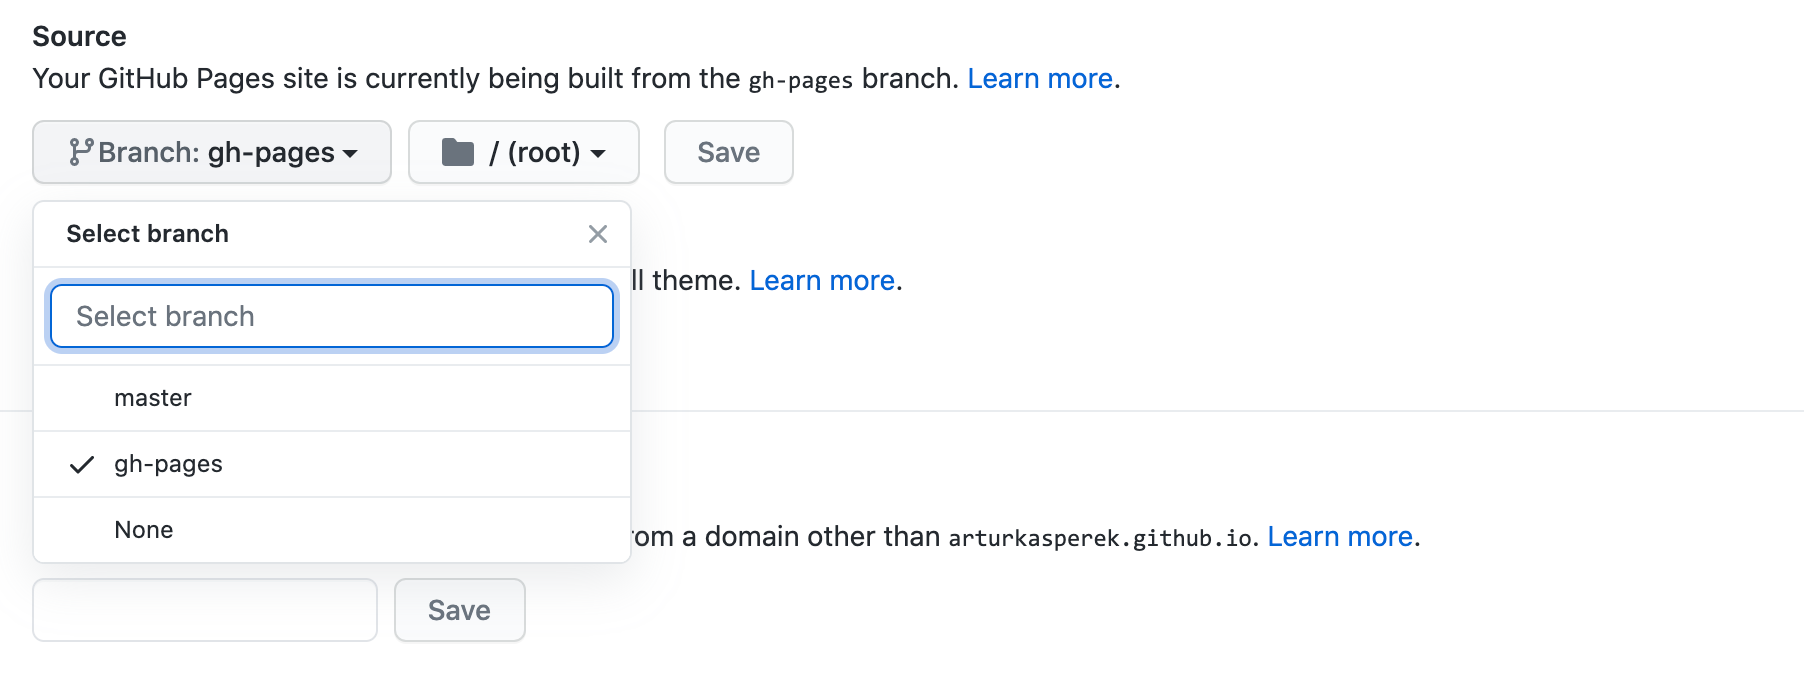
\includegraphics[width=12cm]{gh_pages.png}
  \caption{Ustawienia GitHub Pages}
  \label{fig:gh_pages}
\end{figure}
Dzięki temu będziemy w stanie odseparować gałąź, gdzie trzymamy kod źródłowy strony, od zbudowanej statycznej strony. Jest to także ułatwienie dla potoku automatyzującego. Jeżeli chcielibyśmy zapisywać zbudowaną stronę na gałęzi \textit{master}, oznaczałoby to, że nasz \textit{workflow} wyzwalałby się w nieskończoność przez fakt, iż jest on uzależniony od tego, czy jakieś nowe zmiany zostały wysłane na gałąź \textit{master}.
\par
Definicja tego, co nasz proces ciągłego dowożenia ma robić, wygląda następująco:
\begin{lstlisting}[caption={Definicja zadań \textit{workflow}'a budującego stronę}]
  jobs:
    build-and-deploy:
      runs-on: ubuntu-latest
      steps:
      - uses: actions/checkout@v2
      - name: Use Node.js 14.x
        uses: actions/setup-node@v1
        with:
          node-version: 14.x
      - name: Install Dependencies
        run: |
          yarn install
      - name: Build website
        run: |
          yarn build
      - name: Deploy
        uses: JamesIves/github-pages-deploy-action@3.6.2
        with:
          GITHUB_TOKEN: ${{ secrets.GITHUB_TOKEN }}
          BRANCH: gh-pages
          FOLDER: public
          CLEAN: true
\end{lstlisting}
\par
Jedną z rzeczy, które wyróżniają GitHub Actions nad innymi systemami ciągłej integracji/ciągłego dowożenia, jest możliwość definiowania tytułowych akcji. Akcje to nic innego jak sprytnie zapakowane programy lub też skrypty bash'owe, które pod spodem wykonują jakąś skomplikowaną rzecz. W zależności od argumentów środowiskowych możemy daną akcję dostosować do naszych potrzeb. Z faktu, że każdy może publikować własne akcje, nie jesteśmy ograniczeni do korzystania tylko z akcji dostarczonych przez twórców GitHub Actions. Dzięki takiemu podejściu mamy dostęp do bogatej bazy gotowych modułów.
\par
Wyjaśnijmy teraz, co dane linijki robią. W linii 3 definiujemy to, jaki system chcemy użyć jako bazowy. W naszym przypadku używamy Ubuntu, ponieważ jest najbardziej „lekkim” z wszystkich możliwych systemów. Od linijki 4 do końca mamy definicję kroków, co dany \textit{job} (z ang. \textit{zadanie}) ma wykonać. Pierwszymi krokami jest przełączenie się do danego branch'a oraz użycie akcji, która zainstaluje nam środowisko nodeJS w wersji 14. Od linii 10 do 15 zdefiniowane są dwa kroki, których celem jest zainstalowanie zależności naszego projektu oraz jego zbudowanie. W tym celu używamy menadżera paczek \textit{yarn}, który został zainstalowany dodatkowo podczas instalacji nodeJS. Kroki te pokazują, że nie jesteśmy uzależnieni tylko od użycia gotowych akcji. Za pomocą słowa kluczowego \textit{run} możemy zdefiniować dowolną komendę bash'ową, która ma być wykonana w danym momencie. Warto podkreślić fakt, że zmienne środowiskowe, które były zdefiniowane w danym kroku, nie są dostępne dla kolejnych kroków. GitHub Actions odpala każdy krok w osobnej sesji bash'owej. Na ten moment nasza strona powinna być wybudowana i zapisana w folderze \textit{public}.
\par
Ostanim krokiem jest publikacja strony na gałęzi \textit{gh-pages}. W tym celu używamy gotowej akcji o nazwie \textit{JamesIves/github-pages-deploy-action} w wersji 3.6.2. Jest to przykład akcji, która została dostarczona przez trzeciego autora i jest udostępniona szerokiej publiczności. Akcja ta „pod spodem” za pomocą git'a wysyła dany folder na wyspecjalizowaną za pomocą parametru \textit{BRANCH} gałąź. Dodatkowo musimy podać w parametrach akcji token dostępu do GitHuba. Robimy to za pomocą parametru \textit{GITHUB\_TOKEN}. Token ten jest automatycznie generowany przez GitHub'a podczas odpalania danego \textit{workflow}'a i daje możliwość zapisywania zmian do repozytorium, gdzie \textit{workflow} jest odpalane. Tym sposobem akcja dostaje niezbędne prawa do wysłania folderu z wybudowaną stroną na gałąź \textit{gh-pages}, która jest częścią tego samego repozytorium. Dzięki temu, że wykorzystaliśmy gotową akcję do publikacji naszej strony, ograniczyliśmy długość kodu oraz zredukowaliśmy czas, który musielibyśmy poświęcić na stworzenie skryptu, który wysyła folder \textit{public} na odpowiednią gałąź.
\par
Teraz, gdy nasze repozytorium posiada plik konfiguracyjny GitHub Actions, w zakładce \textit{Action} na GitHub'ie powinniśmy zauważyć zakolejkowane zadanie budowania strony.
\begin{figure}[htbp]
  \centering
  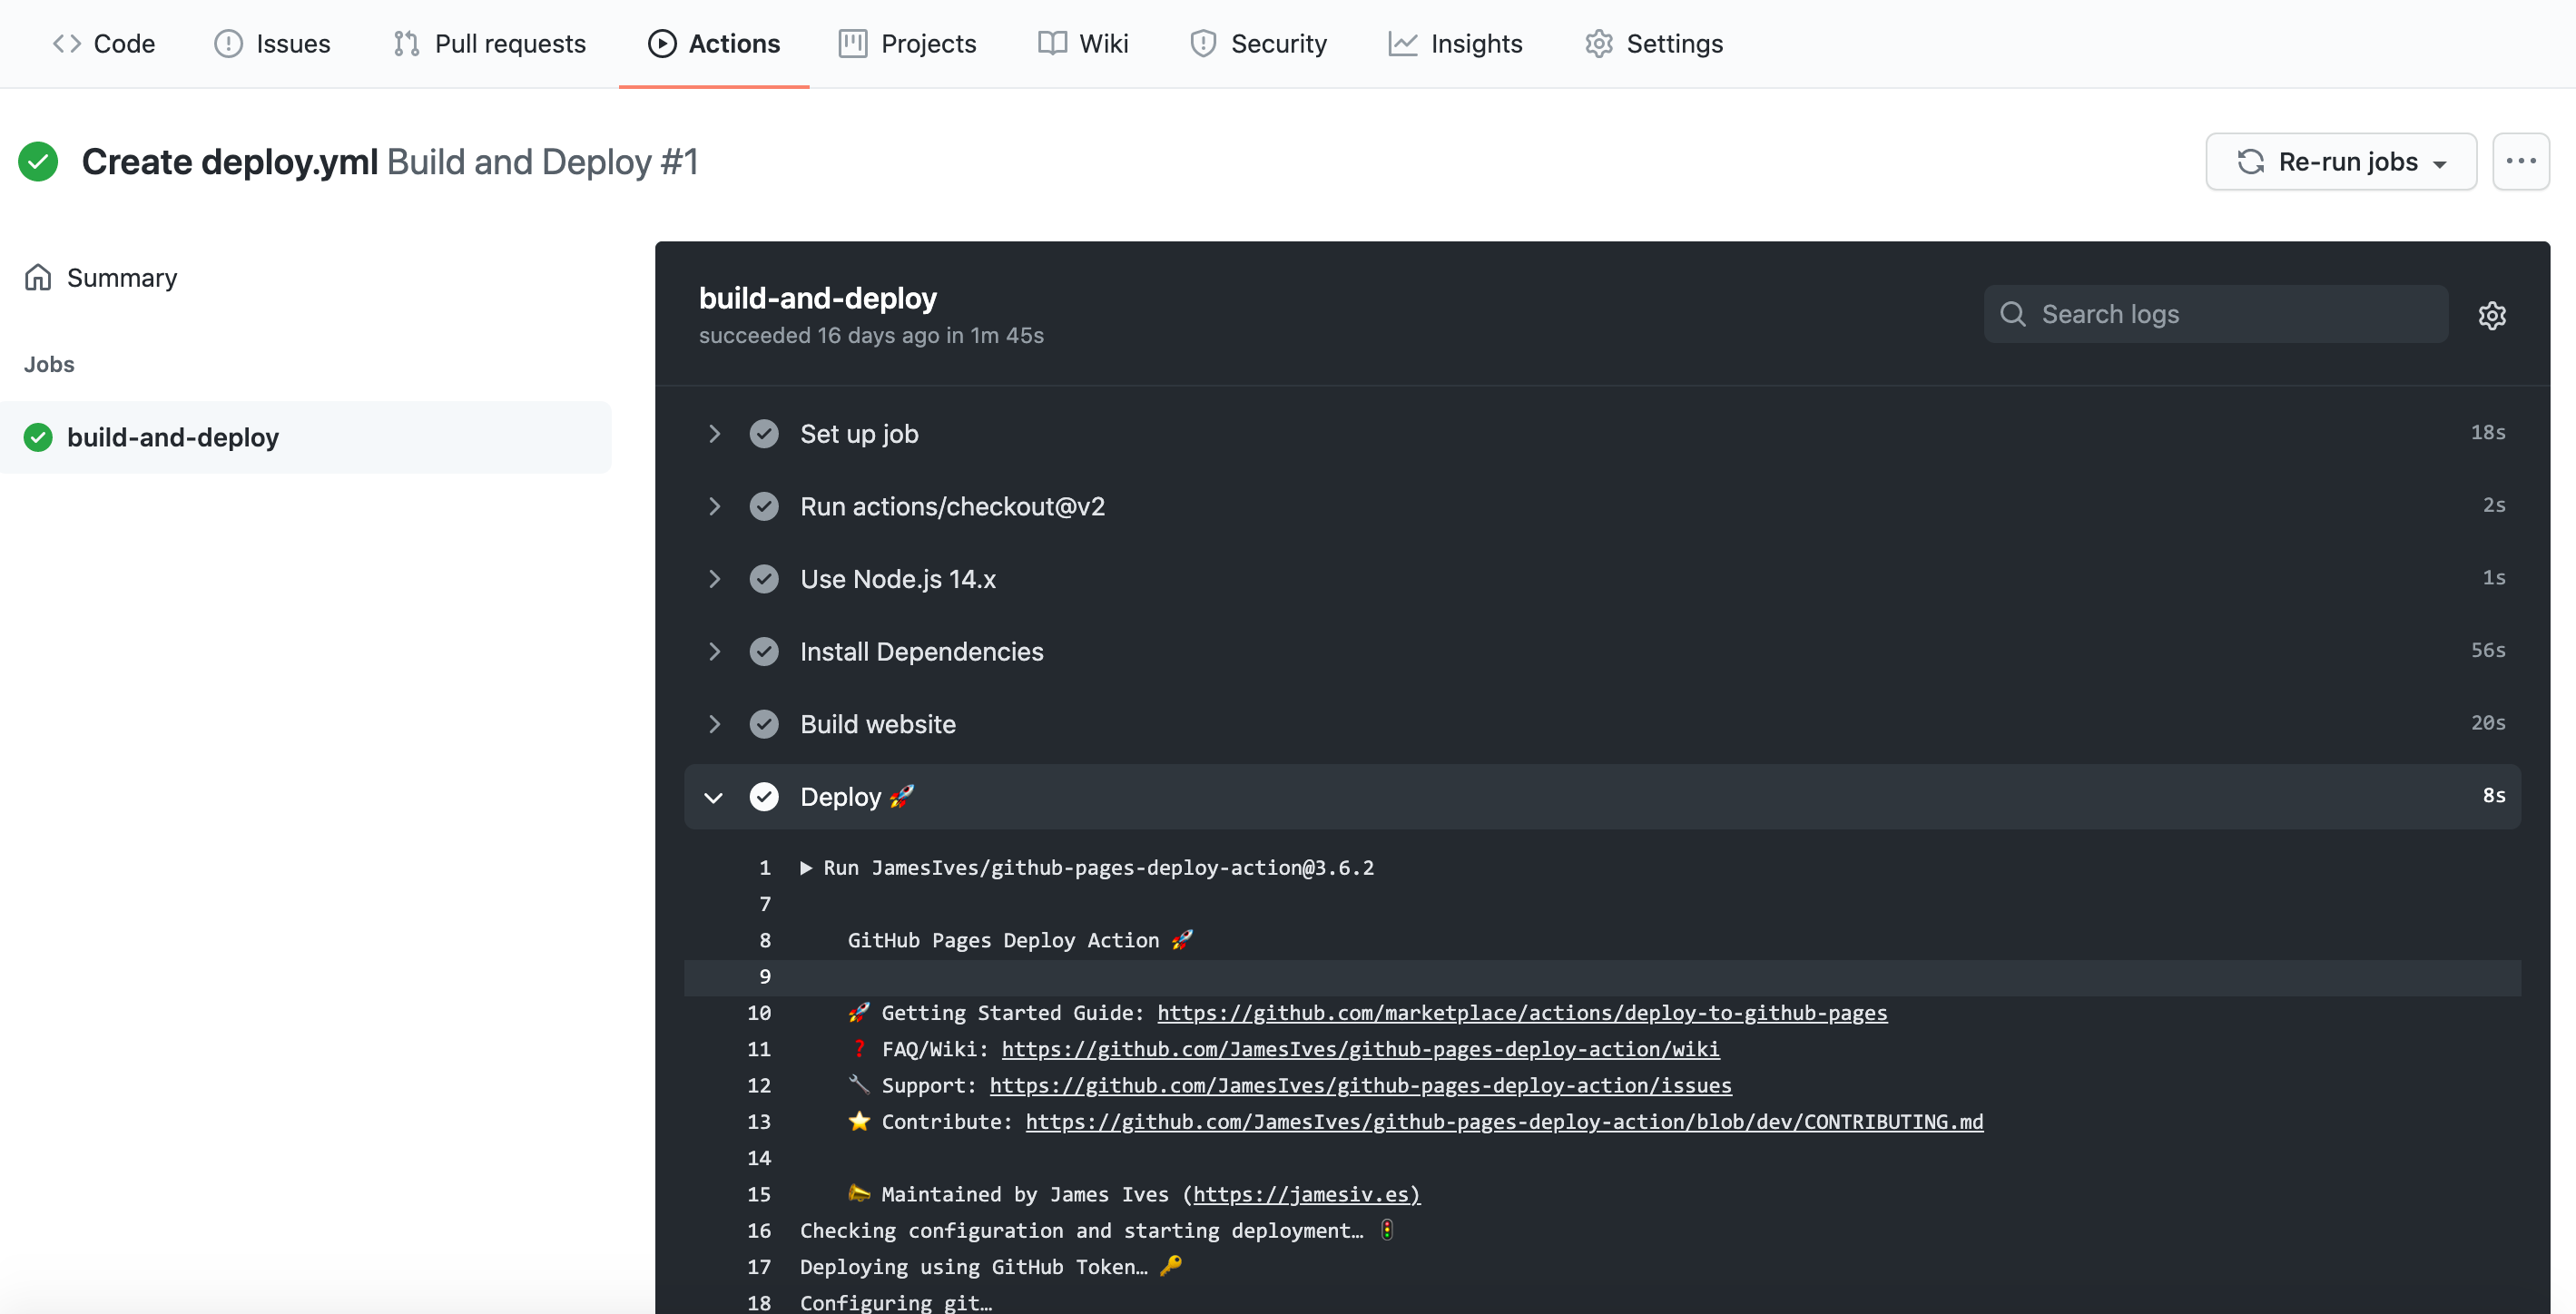
\includegraphics[width=12cm]{gh-actions-log.png}
  \caption{Widok na którym możemy zobaczyć szczegóły danego zadania}
  \label{fig:gh_actions_log}
\end{figure}
Sumarycznie pierwsze budowanie strony zajęło 1min 45sec. Najwięcej czasu zabrało zainstalowanie zależności - aż 56 sekund. Na szczęście GitHub zapewnił akcję, która pozwala cache'ować zależności. Warunkiem koniecznym do działania tego mechanizmu jest posiadanie pliku z informacjami o wersjach zależności jakich używamy. Nie powinno być to problemem, ponieważ większość współczesnych menadżerów zależności generuje taki plik. Implementując cache'owanie, proces automatyzujący będzie tylko instalował zależności, jeżeli jakaś ich wersja się zmieni - w reszcie przypadków proces używa plików z cache'a.
\par
Po tym, gdy pliki z stroną „wylądowały” na gałęzi \textit{gh-pages}, GitHub powinien zakolejkować proces publikacji strony. Jest to rzecz, nad którą nie mamy kontroli.
\begin{figure}[htbp]
  \centering
  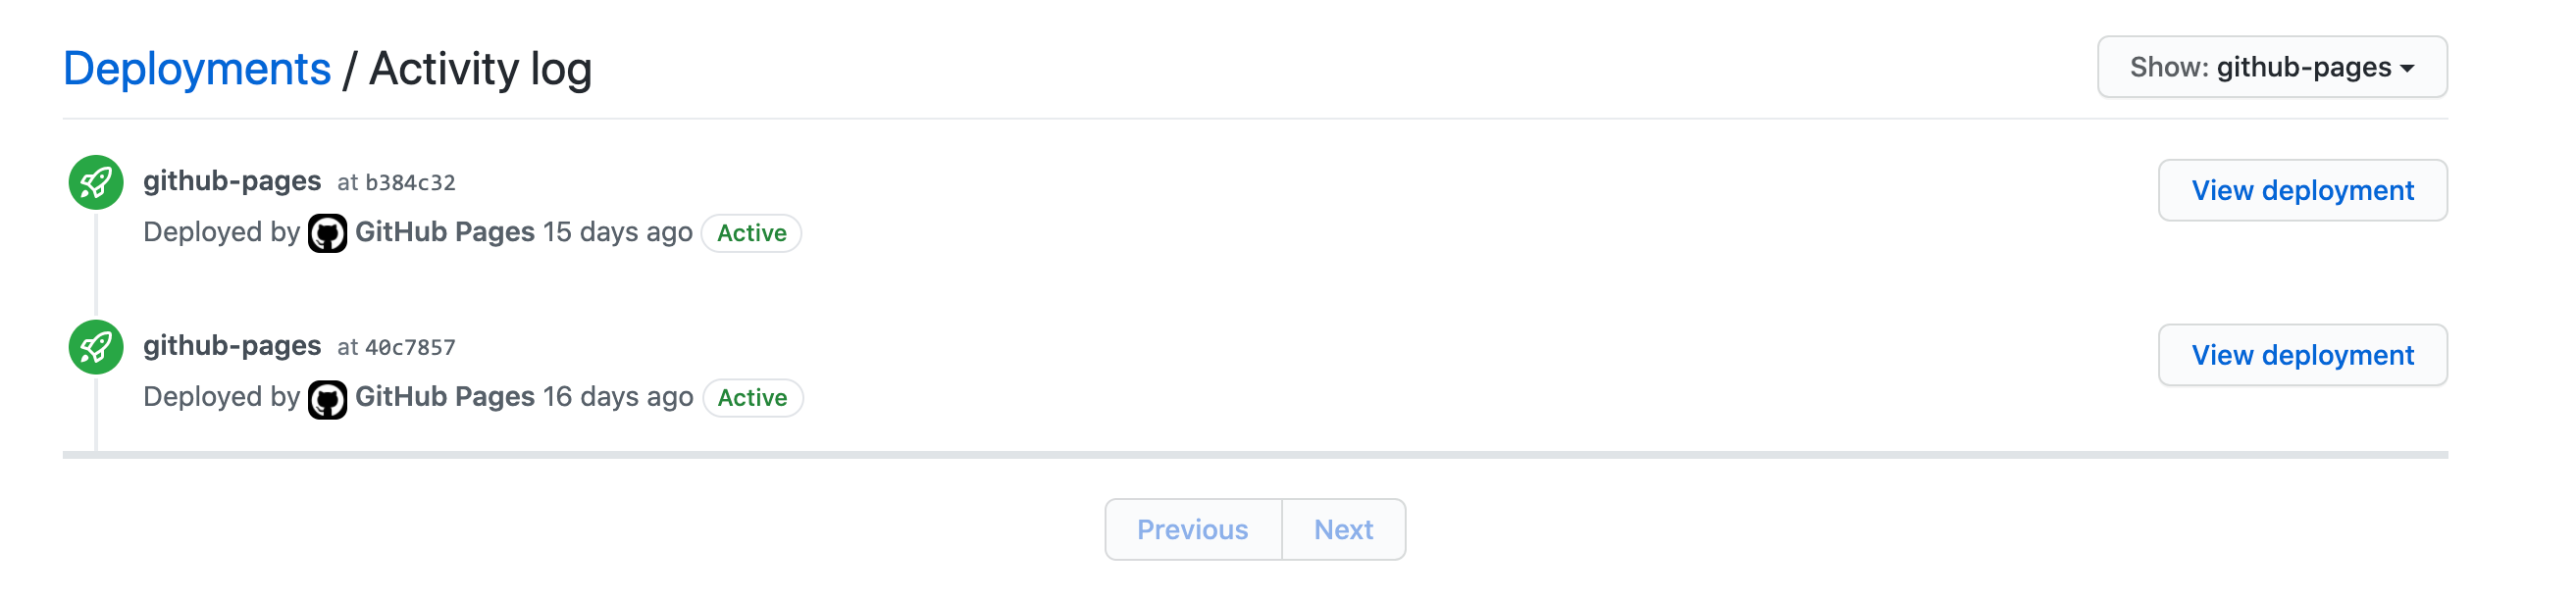
\includegraphics[width=12cm]{gh_pages_deploy.png}
  \caption{Widok z publikacjami strony}
  \label{fig:gh_pages_deploy}
\end{figure}
\par
GitHub wewnętrznie bierze pliki strony z gałęzi, którą ustawiliśmy, i publikuje to na swoich serwerach. Finalnie omawiana strona jest dostępna pod adresem \textit{https://arturkasperek.github.io/static-website-with-ci-cd/}. GitHub pages samo w sobie nie ogranicza nas do używania domeny \textit{github.io}. Jeżeli posiadamy własną domenę, możemy odpowiednio tak przekierować ruch do GitHub'a, że finalny użytkownik nie będzie wiedział, gdzie strona jest hostowana.
\par
Dzięki zapewnieniu modułowości, GitHub Actions może pochwalić się dużą biblioteką akcji stworzoną przez społeczeństwo. Oto lista ciekawych akcji:
\begin{itemize}
  \item jakejarvis/s3-sync-action - jest to akcja, która pozwala synchronizować dany folder repozytorium z folderem na usłudze hostingowej AWS S3. Może być użyteczna, jeżeli chcielibyśmy danej grupie deweloperów dać możliwość wysyłania plików na S3, bez konieczności dawania dostępu do panelu administratora AWS,
  \item repo-sync/github-sync - akcja ta potrafi synchronizować dane repozytorium z innym repozytorium dostępnym w sieci. Jest ona szczególnie użyteczna, gdy pracujemy nad fork'iem (fork to kopia projektu która rozwija się niezależnie względem oryginału) jakiegoś projektu i chcemy utrzymać zgodność z oryginałem. GitHub Actions pozwala na odpalanie danego procesu automatyzującego automatycznie na podstawie planera. Dzięki temu możemy wykorzystać tą akcję, by co jakiś czas synchronizowała nasze repozytorium z macierzystym projektem,
  \item release-drafter/release-drafter - akcja jest szczególnie użyteczna, jeżeli nasz projekt chce korzystać z dobrych praktyk, dotyczących publikacji oprogramowania. Akcja ta oblicza, jakie zmiany w kodzie nastąpiły od ostatniej publikacji i tworzy wstępną publikację na GitHub'ie z opisem zmian, które dokonaliśmy. Akcja ta jest oparta na commit'ach, dlatego warto by one były dobrze opisane. Jeżeli użyjemy odpowiednich prefixów jak \textit{feature} oraz \textit{bug}, akcja będzie w stanie lepiej sformatować opis publikacji,
  \item zaproxy/action-baseline - jest to akcja, która jest oparta o użycie narzędzia ZAP - to program, który analizuje nasz kod pod względem różnorakich luk bezpieczeństwa. Finalnie jeżeli akcja w wyniku swojego działania znajdzie jakieś podatności to tworzy automatycznie \textit{issue} (system na GitHub'ie, który pozwala śledzić błędy). Jest to ciekawa opcja, jeżeli chcemy jak najbardziej zabezpieczyć się przed ewentualnymi atakami hackerów.
\end{itemize}
Wszystkie powyższe rzeczy moglibyśmy wykonać, używając akcji, która odpala skrypt bash'owy. Takie podejście jednak miałoby sporo wad - bylibyśmy zmuszeni spędzić sporo czasu, by wszystko zgrać tak jak chcemy. Dodatkowo prawdopodobnie nie pokrylibyśmy różnych przypadków brzegowych. Dzięki gotowym akcjom czas konfiguracji środowiska do automatyzacji skraca się do minimum, a my możemy się skupić na rozwiązywaniu innych problemów.



% tutaj mógłbym rozwinąć rozdział 3 i powiedzieć, że coraz mniej używa się Jenkinsa i obecnie popularne są platformy jak Github Actions, CircleCI czy gitlabCI, które są trigerrowane przez commity, pushe czy też tworzenie tagów z pomocą systemu wersji git. Myślę, że mógłbym tutaj zrobić nawiązanie do części praktycznej pracy:
% 4a) continues delivery w React Native na przykładzie GitHub actions
% 4b) continues deploymeny na przykładzie aplikacji backendowej w javaScriptcie
% 4c) continues deployment strony internetowej hostowanej przez GitHub actions za pomocą circleCI
% W każdym z tych podrozdziałów opisałbym jaki jest ogólny problem i dalej opisałbym już konkretne rozwiązanie
